\documentclass[acmtocl,acmnow]{acmtrans2m}
\usepackage{amscd}
\usepackage{amsmath}
\usepackage{amsfonts}
\usepackage{graphicx}
\usepackage{listings}
\usepackage{color}
\usepackage[vlined,algoruled]{algorithm2e}

\newtheorem{theorem}{Theorem}[section]
\newtheorem{conjecture}[theorem]{Conjecture}
\newtheorem{corollary}[theorem]{Corollary}
\newtheorem{proposition}[theorem]{Proposition}
\newtheorem{lemma}[theorem]{Lemma}
\newdef{definition}[theorem]{Definition}

\newcommand{\proj}{\textrm{\textbf{Proj}} } 
\newcommand{\tr}{\textrm{trace}} 
 
\lstset{ %
  language=C++,                % the language of the code
  basicstyle=\footnotesize,           % the size of the fonts that are used for the code
  numbers=left,                   % where to put the line-numbers
  numberstyle=\tiny\color{gray},  % the style that is used for the line-numbers
  stepnumber=1,                   % the step between two line-numbers. If it's 1, each line 
                                  % will be numbered
  numbersep=5pt,                  % how far the line-numbers are from the code
  backgroundcolor=\color{white},      % choose the background color. You must add \usepackage{color}
  showspaces=false,               % show spaces adding particular underscores
  showstringspaces=false,         % underline spaces within strings
  showtabs=false,                 % show tabs within strings adding particular underscores
  frame=single,                   % adds a frame around the code
  rulecolor=\color{black},        % if not set, the frame-color may be changed on line-breaks within not-black text (e.g. commens (green here))
  tabsize=2,                      % sets default tabsize to 2 spaces
  captionpos=b,                   % sets the caption-position to bottom
  breaklines=true,                % sets automatic line breaking
  breakatwhitespace=false,        % sets if automatic breaks should only happen at whitespace
  title=\lstname,                   % show the filename of files included with \lstinputlisting;
                                  % also try caption instead of title
  keywordstyle=\color{blue},          % keyword style
  commentstyle=\color{dkgreen},       % comment style
  stringstyle=\color{mauve},         % string literal style
  escapeinside={\%*}{*)},            % if you want to add a comment within your code
  morekeywords={*,...}               % if you want to add more keywords to the set
}

\newdef{remark}[theorem]{Remark}

%\markboth{XXX}{YYY}
\title{\textbf{A virtual reality setup made easy}}
            
\author{Carlo Nicolini\\Center for Cognitive Neuroscience CNCS\\Istituto
Italiano di Tecnologia}
            
\begin{abstract}
We present a virtual reality system simple to build and to maintain. The system allows real-time virtual reality head tracking only with a tracking system and a computer.
We believe this system can apply to a variety of psychophysics experiment where one has to know the position of the observer. It also allows a replay of the scene as view from the observer (passive observer).
\end{abstract}

\keywords{Virtual reality, computer graphics}

\begin{document}
\begin{bottomstuff}
Author's address: Carlo Nicolini, Center for Cognitive Neuroscience CNCS,
Istituto Italiano di Tecnologia (IIT),
Corso Bettini 31, Rovereto, Italy
\end{bottomstuff}

\maketitle

\section{Introduction and motivation}
Doing experiments in visual perception where the subject is inside a virtual reality environment usually requires a lot
of programming of the head tracking system, calibration and visual stimuli presentation and for the inexperienced programmer this is often a long process.

In response to this need an object-oriented simulation toolkit \textit{CNCSVision} has been developed. The toolkit provides a diverse, wide-ranging, yet cohesive set of software components which can be employed in a variety of experimental settings.
\section{Previous works}
\begin{itemize}
 \item Articolo Panerai - svantaggi - vantaggi - modello meccanico - precisione - limitatezza nel display - noi sfruttiamo la pipeline della scheda grafica per lavorare sui vertici => stimoli qualsiasi
 \item Confronto con articoli di realtà virtuale e percezione visiva dove fanno cose più fiche graficamente
 \item Differenze con gli head-mounted display (come funziona la disparità con tali display? vergenza-accomodazione inconsistenti con distanze simulate) articoli che citano questo problema
\end{itemize}
SPECIFICHE TECNICHE MINIME PER RICREARE IL SETUP:
Requisiti minimi - 
sistema creato con 1) optotrak NDI 2) computer+schermo 3) shutter glasses

Rispetto agli altri abbiamo un grado di libertà (roll) in più che permette un passivo più completo.

\section{Model of an observer in VR}

We must understand and decide what to model mathematically when a person moves inside an environment looking to objects and interacting with them.
In order to reconstruct what a person is viewing at a given time, we must know the person position and orientation with respect to a given reference frame.

In the following section we will use $\mathbb{E}^3$ to denote the familiar three-dimensional Euclidean space\footnote
{
We will denote common three-dimensional vectors with lowercase bold letters $(\mathbf{x}, \mathbf{p})$, unit-norm three dimensional vectors with 
lowercase bold letters and a hat: $\mathbf{\hat{u}},\mathbf{\hat{v}}$,  matrices with uppercase bold letters $(\mathbf{A}, \mathbf{B})$, identity matrix with $\mathbf{I}$,
 scalars with lowercase letters $a,b,c$. We will use the same convention for points and vectors whenever their correct dimensions is clear from the context.
} we follow the notation of \cite[Soatto]{Ma:2003:IVI:971144},every point $\mathbf{x} \in \mathbb{E}^3$ can
be identified with a point in $\mathbb{R}^3$ with three coordinates $$\mathbf{x} = [x,y,z]^T.$$

We choose two reference frames, the global frame $O$ and the local frame $O'$ and a invertible map $H : O \rightarrow O'$: a real-world observer can then be described as a local reference frame in global coordinates.
The transformation from global to local reference frame takes the form of an affine transformation, consisting of a rotation and a translation.

Coordinates of a point $\mathbf{x}=(x,y,z)$ in $O$ undergo the transformation law described by the map $H$ such that: $\mathbf{x}' = H( \mathbf{x})$. A rigid-body transformation is a special kind of 
map which is composed by a rotation described by a $\mathbb{R}^{3\times 3}$ orthogonal matrix\footnote{A matrix belonging to $SO(3)$ group, i.e holds $\mathbf{R}^{-1}=\mathbf{R}^T$ and $\det{R}=1$} and a translation described by a $\mathbb{R}^3$ displacement vector such that:
\begin{equation}
\label{eq:affinemotion}
 \mathbf{x}' = \mathbf{R} \cdot \mathbf{x} + \mathbf{t}
\end{equation}
An affine transformation of this kind can be regarded as ``rigid-body'' transformation because
it preserves distances between points.

In order to describe the rigid-body motion one should in
principle specify the trajectory of every single point on the object but
fortunately for rigid objects we do not need to specify the
motion of every point, it's sufficient to specify the motion of one and the
motion of three coordinate axes attached to it, because the distance
between any points on it does not change over time as the object moves.

A rigid-body motion can be described at every temporal instant $t > t_0$ by a $3\times
3$ rotation matrix $\mathbf{R}(t) \in \mathbb{R}^{3\times 3}$ and a displacement
vector $\mathbf{t}(t) \in \mathbb{R}^{3}$ such that for every point $\mathbf{x}_i$ on
the rigid body the following relation holds:
\begin{equation}\label{eq:affinemotion2}
  \mathbf{x}_i(t) = \mathbf{R}(t)\cdot \mathbf{x}_i(t_0) + \mathbf{t}(t)
\end{equation}

We note that the coordinates transformation for a rigid body motion is not
linear but \emph{affine}, nonetheless we may convert such an 
affine transformation to a linear one by using homogeneous coordinates appending
$'1'$ to the coordinates of a point $\mathbf{x} \in \mathbb{E}^3$ yielding
a vector  in $\mathbb{R}^4$. Using the $4$ dimensional notation, we can rewrite (\ref{eq:affinemotion}) in a linear fashion

\begin{align}\label{eq:homogenized}
\mathbf{x}_i(t) = \mathbf{H} \cdot \mathbf{x}_i(t_0)
\end{align}

where the matrix $\mathbf{H}\in \mathbb{R}^{4\times 4}$ represent the invertible map $H$:

\begin{align*}
\mathbf{H} = \begin{bmatrix} \mathbf{R} & \mathbf{t} \\ \mathbf{0} & 1
\end{bmatrix}
\end{align*}
and is called the
\emph{homogeneous representation} of the rigid-body motion. This allows us to describe rigid-body motion as linear matrix-vector multiplication.
%Now that we have a theoretical framework to describe observer in an environment and change of coordinates, we focus on the way computers represent three-dimensional world.

\subsection{Generalized perspective projection}
So far we have used affine transformations as a method for displacing objects in Euclidean space.

We now turn our attention to perspective projection stage in which the Euclidean space is represented on a two-dimensional zero-curvature surface.

The projection stage places a camera or eye with a given position, view direction, and field of view.
The camera is modeled as a reference frame with 6 degrees of freedom which determine the parts of the three-dimensional model in the final image.

Camera transformations involve not only affine transformation but also perspective transformations. This kind of transformations are needed to make three-dimensional points render on a screen as 
pixel coordinates along with color and depth coordinates.

Unfortunately, while perspective projection is a well understood method in computer graphics \cite[Buss]{Buss:2003:CGM:861813}, it make some assumptions that are not valid for an head-tracking system.
Here we generalize the standard perspective projection in a general fashion \cite[Kooima]{kooima}. We'll also obtain a correct stereoscopic system with a minimum effort.

From now on we'll treat point in global reference frame $O$ and omit the uppercase $O$ in the vectors and call ``right'' the positive $x$ axis, ``up'' the positive $y$ axis and toward the negative $z$ axis.
Let us fix a global reference frame $O_{xyz}$ and define three points $\mathbf{p}_{a}$, $\mathbf{p}_b$, $\mathbf{p}_c$ lying respectively on the lower left, lower
right and upper left corners of a rectangle.

These points are used to compute an orthonormal basis in $O$  called $(\mathbf{v}_r$,
$\mathbf{v}_u$,$\mathbf{v}_n)$ for the screen space\footnote{Loosely speaking,
the unit vectors of the screen space orthonormal basis give us a basis for
describing points relative to the screen.}:
\begin{eqnarray}
 \mathbf{v}_r = \frac{\mathbf{p}_b-\mathbf{p}_a}{||\mathbf{p}_b-\mathbf{p}_a||}
\nonumber \\
 \mathbf{v}_u = \frac{\mathbf{p}_c-\mathbf{p}_a}{||\mathbf{p}_c-\mathbf{p}_a||}
\nonumber \\
 \mathbf{v}_n = \frac{\mathbf{v}_r \times \mathbf{v}_u}{||\mathbf{v}_r \times
\mathbf{v}_u||}
\end{eqnarray}

Let's consider a point $\mathbf{p}_e$ called COP (center of projection) which will represent the eye of the observer in our setup.
 
Here we want to allow the COP to move freely having the correct perspective computed. Let $d$ be the distance from COP to the rectangle surface:
\begin{equation}
 d = - \mathbf{v}_n \cdot ( \mathbf{p}_a -\mathbf{p}_e )
\end{equation}

 \begin{figure}[ht]
 \centering
 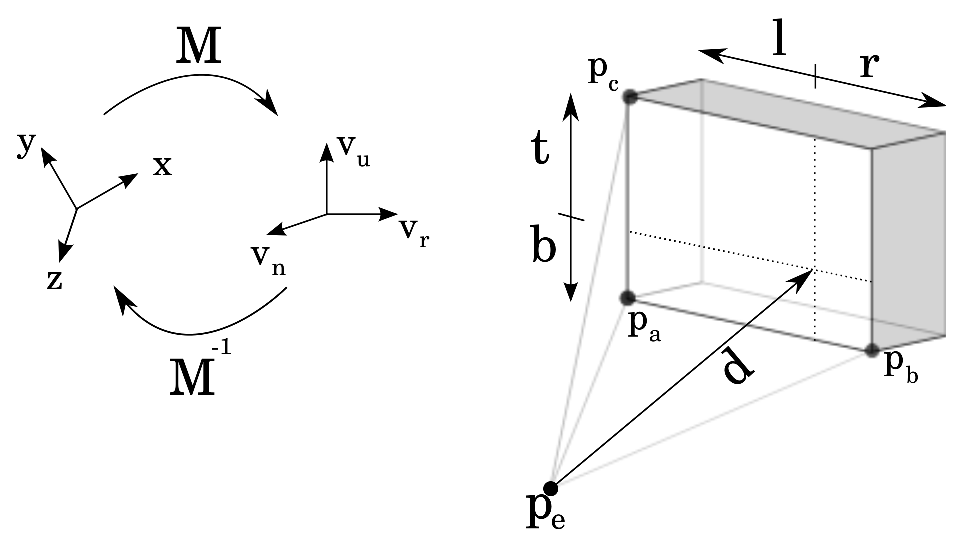
\includegraphics[width=0.6\textwidth]{genperspectiveprojection2.eps}
 % perspectiveprojection.ps: 596x842 pixel, 72dpi, 21.03x29.70 cm, bb=0 0 596 842
 \caption{Generalized perspective projection scheme with meaning of each
variable.}
 \label{fig:perspectiveprojection}
\end{figure}

It can be shown that the scalars $\{l,r,t,b\} \in \mathbb{R}$ are the frustum extents and are needed for perspective projection. They are given by the following relations:

\begin{eqnarray*}
& l = \dfrac{n(\mathbf{v}_r \cdot \mathbf{v}_a )}{d} &\hspace{6mm} r = \dfrac{n(\mathbf{v}_r
\cdot \mathbf{v}_b )}{d} \nonumber \\
& b = \dfrac{n(\mathbf{v}_u \cdot \mathbf{v}_a )}{d} &\hspace{6mm} t = \dfrac{n(\mathbf{v}_r
\cdot \mathbf{v}_c )}{d} 
\end{eqnarray*}
where $n,f$ are the depth extensions of the frustum and 
\begin{eqnarray*}
\mathbf{v}_a  = \mathbf{p}_a - \mathbf{p}_e \nonumber \\ 
\mathbf{v}_b  = \mathbf{p}_b - \mathbf{p}_e \nonumber \\
\mathbf{v}_c  = \mathbf{p}_c - \mathbf{p}_e \nonumber \\
\end{eqnarray*}
We form the perspective projection matrix $\mathbf{P}\in \mathbb{R}^{4 \times 4}$ then as
follows:
\begin{align}
\mathbf{P}= \begin{bmatrix}
\dfrac{2n}{r-l} & 0 & \dfrac{r+l}{r-l} & 0 \\ 
0 & \dfrac{2n}{t-b} & \dfrac{t+b}{t-b} & 0 \\ 
0 & 0 & -\dfrac{f+n}{f-n} & -\dfrac{2fn}{f-n} \\ 
0 & 0 & -1 & 0 
\end{bmatrix}
\end{align}

The matrix $\mathbf{P}$ now represents a frustum lying with the front plane on the $XY$ plane.
To allow a general treatise of the screen as projection surface (and then distinguish between \emph{active} and \emph{passive} display as we'll see later on) we have to find a transformation which accounts both for the rotation and for 
the translations relative to the canonical base in the target frame.

Since we are working in homogenized coordinates, let's introduce $\mathbf{M}$:

\begin{align*}
\mathbf{M} =
\begin{bmatrix}
\mathbf{R}_M & 0 \\
\mathbf{0} & 1 
\end{bmatrix}
=
\begin{bmatrix}
v_{rx} & v_{ux} & v_{nx} & 0 \\
v_{ry} & v_{uy} & v_{ny} & 0 \\
v_{rz} & v_{uz} & v_{nz} & 0 \\
0 & 0 & 0 & 1
\end{bmatrix}
\end{align*}

Recall that when we want to rotate our frustum to align it within our
tracker space we instead rotate our tracker space to align it with our frustum.
With the orthogonality of $\mathbf{M}$ in mind, the right matrix to apply to $\mathbf{P}$ is $\mathbf{M}^T$.

A last point in the creation of the generalized perspective projection matrix is keeping in account for the COP position. This is accomplished with a last
multiplication by a $4 \times 4$ translation matrix $\mathbf{T}$:
\begin{align*}
\mathbf{T} =
\begin{bmatrix}
1 & 0 & 0 & -p_{e_x} \\
0 & 1 & 0 & -p_{e_y} \\
0 & 0 & 1 & -p_{e_z} \\
0 & 0 & 0 & 1 
\end{bmatrix}
\end{align*}
Finally the generalized perspective matrix to be used in a active vision
experiment with head tracking is the following:
\begin{equation}
\mathbf{P'} = \mathbf{P} \cdot \mathbf{M}^T \cdot \mathbf{T}
\end{equation}
This model simply extends to two alternate centers of projection, leading to a correct stereopsis.

\section{Extracting coordinates}
While in theory is possible to track the COP position, in a real-world head tracking system this is not possible usually being the COP coincident with the eyes of the subject. We propose an approach to estimate 
COP as well as other points by mean of rigid-body transformations.

It's possible to estimate the before discussed rigid body transformation matrix $\mathbf{H}(t)$ given two sets of at least $3$ points for which corresponding pairs have been determined. This problem is known 
in literature as the \emph{absolute orientation problem}. We tackle the problem using \emph{Umeyama}'s method \cite{umeyama} being the most reliable and stable.

% Due to its ubiquity, in the next sections we'll refer to the Umeyama algorithm as that function with input the two set of points (source and destination) and as output the \emph{rigid-body motion matrix} $\mathbf{H}$:
% \begin{equation}
%  \mathbf{H} = \textrm{umeyama}\left( \mathbb{X}_{\textrm{src}}, \mathbb{X}_{\textrm{dst}} \right)
% \end{equation}

Umeyama method estimates both parameters $\tilde{\mathbf{R}}$ and $\tilde{\mathbf{t}}$ of rigid-body transformation $\mathbf{H}$ (and an
additional scaling parameter $c\in \mathbb{R}$) by minimizing a mean squared error $e^2(\tilde{\mathbf{R}},\tilde{\mathbf{t}},c)$ of two set of points:
\begin{equation}\label{eq:umeyama}
e^2(\tilde{\mathbf{R}},\tilde{\mathbf{t}},c) = 
 \dfrac{1}{N}  \sum \limits_{i=0}^N \begin{Vmatrix} \mathbf{x}_{i}(t_0)
-c(\tilde{\mathbf{R}} \cdot \mathbf{x}_i(t) + \tilde{\mathbf{t}}) \end{Vmatrix}^2
\end{equation}
where in our case we set the number of destination and source points $N>3$ and $c=1$ \cite{umeyama,DBLP:books/daglib/0086372}. 

In this following analysis $\mathbf{H}$ allows to implement the 3-D rigid transformation from \emph{source} to \emph{destination} points as an efficient matrix-vector multiplication:
\begin{equation}
 \mathbf{x}_i(t) =  \mathbf{H}(t)\cdot \mathbf{x}_i(t_0) = \begin{bmatrix} \mathbf{R} & \mathbf{t} \\ 0 & 1\end{bmatrix} \begin{bmatrix} \vec{\mathbf{x}_i}(t_0) \\ 1\end{bmatrix}\qquad \forall
i=1,\ldots,N
\end{equation}
where $\mathbf{x}_i(t_0), \mathbf{x}_i(t) \in \mathbb{R}^4$ and $\vec{\mathbf{x}_i}(t_0)\in \mathbb{E}^3$. This methods helps to track points which are not under the detectable space of a tracking system by interpolation.

\emph{Ghost points} are here referred as those points in the VE without a
physical counterpart (basically a physical marker representing it), but which are computed from another set of point (reference). They will always be denoted
 with a tilde, e.g. $\tilde{\mathbf{x}}$. A \emph{ghost point} is a central concept, because it give more degrees of freedom to the user, allowing him to move freely in the space, without bothering
about physical markers occlusion due to obstacles in the optic path from the camera to the emitting diode\footnote{We call a marker in the optical range of the tracking system a \emph{visible} marker, \emph{non-visible} otherwise}.
They can be estimated given a relation with at least three reference points.

Let's define two ordered set of points, the first acting as
\emph{reference}: $\mathbb{X}_{\textrm{ref}} = \{
\mathbf{x}_1,\mathbf{x}_2,\mathbf{x}_3 \}$,
and the second $\mathbb{X}_{\textrm{image}} =\{ \mathbf{x}_i \}$ with $i=4,\ldots,N$
containing the starting points $\mathbf{\tilde{x}}_{i}$  which will
undergo the rigid-body transformation $\mathbf{H}$.

The ghost points  $\tilde{\mathbf{x}}_i(t)$ are then calculated when the motion parameters matrix
$\tilde{\mathbf{H}}$ is extracted by applying the absolute orientation problem to the
two sets of reference points $\mathbb{X}_{\textrm{ref}}(t_0)$ and $\mathbb{X}_{\textrm{ref}}(t)$ obtaining the central equation for ghost-point estimation:
\begin{equation}
	\tilde{\mathbf{x}}_i(t) = \tilde{\mathbf{H}}(t)\cdot \mathbf{x}_i(t_0) \quad
\forall i=4,\ldots,N
\end{equation}

We verified the goodness of the method in the points reconstruction by checking that the distance of a real point and its computed equivalent ghost point is always less than $0.5$ mm (mettere qualche grafico o misura?).

\section{Passive observer}
By only mean of matrix transformations is simple to reproduce the geometry as projected to the moving COP but for a static observer.

In an active vision experiments we distinguish between \emph{active} and \emph{passive display}. In our terms, an \emph{active display}, is one in which the frustum holds 
still in a global frame of reference so that $\mathbf{M}(t) = \mathbf{M}(t_0)$ but $d=d(t)$, while a \emph{passive display}, is instead the one in which the projection 
surface rotates so that $\mathbf{M}=\mathbf{M}(t)$ keeping its normal vector always parallel to observer and the distance $d$ constant.

This kind of view display can be simply obtained within this framework by
transforming the screen corners with the estimated \emph{head transformation matrix}
$\tilde{\mathbf{H}}$ and applying what described before for the new screen corners
$\mathbf{p}'_{\{a,b,c \}}$
\begin{eqnarray}
\mathbf{{p}'}(t)_{\{a,b,c\}} = \tilde{\mathbf{H}}(t) \cdot \mathbf{p}_{\{a,b,c\}}
\end{eqnarray}
This equation keeps the virtual screen borders always fronto-parallel to the face of the subject and allows to study the retinic image.

\section{Manipulating stimuli}

Investigation of phenomena in visual perception of structure from motion needs specific visual stimuli. By mean of geometric manipulation we are able to present visual stimuli made of simple random 
pattern of points, for different study situations. Before showing the details of stimuli positioning we introduce the Euler angles convention we'll use when describing
subject rotation in the experimental setup:
\begin{itemize}
 \item Yaw is the angle around the axis from feet to the head of a standing person.
 \item Roll is the angle around the axis from to nape to nose.
 \item Pitch is the angle around the axis from left to right shoulders.
\end{itemize}


\begin{figure}[htb]
 \centering
\caption{Illustration of the three principal euler angles $(y,x,z)$ convention.}
 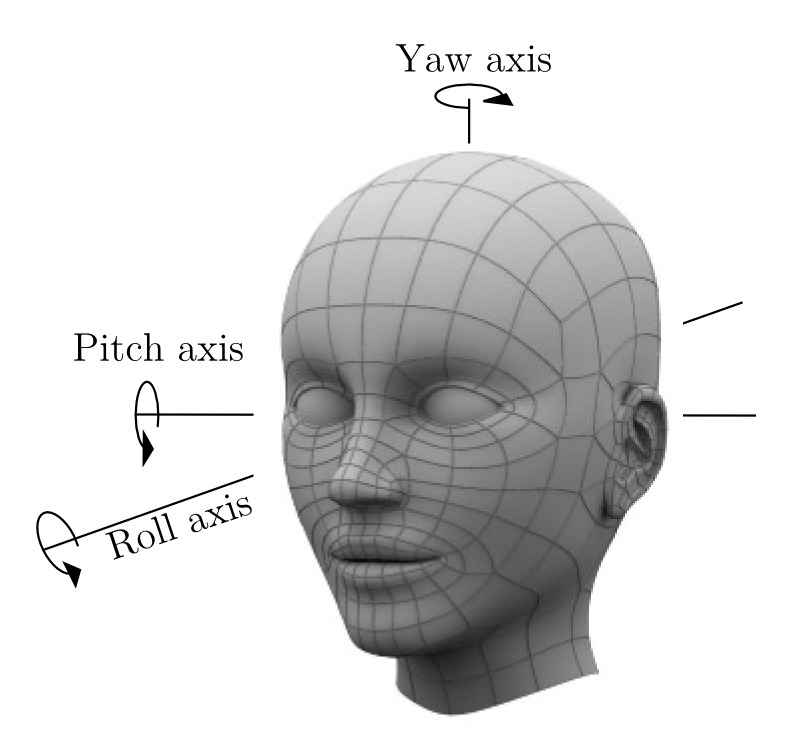
\includegraphics[bb=0 0 162 150]{images/head-yaw-roll-tilt.jpg}
 % head-yaw-roll-tilt.jpg: 807x754 pixel, 201dpi, 10.22x9.54 cm, bb=0 0 290 271
\end{figure}

\subsection{Simple rotating plane}
In order to present a stimulus with the same yaw of the subject head we first must align the subject head at rest with the global reference frame and setting the identity head transformation matrix 
when he's sitting feeling comfortable, facing toward the negative z axis with vanishing $\hat{xz}$ and $\hat{yz}$ angles and then rotate the stimulus accordingly to the yaw angle of the resulting head transformation matrix.
We position the visual stimulus, a plane of random red dots, on the focal plane, with its center in the point $(0,0,f_z)$ in order to eliminate parallax and let it rotate around the $y$ axis as in figure 

The stimulus transformation will be then a composition of a translation $T(\mathbf{x})$ and a rotation $M(\mathbf{x})$: $T \circ M$, in matrix notation a multiplication $\mathbf{M}_s = \mathbf{T}_s \cdot \mathbf{R}_s$.
We can simulate faster or slower rotation of the plane w.r.t head yaw, by putting a multiplicative constant $k$ to the yaw.
\begin{figure}[htb]
% \centering
\label{fig:planeyaw}
\caption{Illustration of simple rotating plane experiment.}
 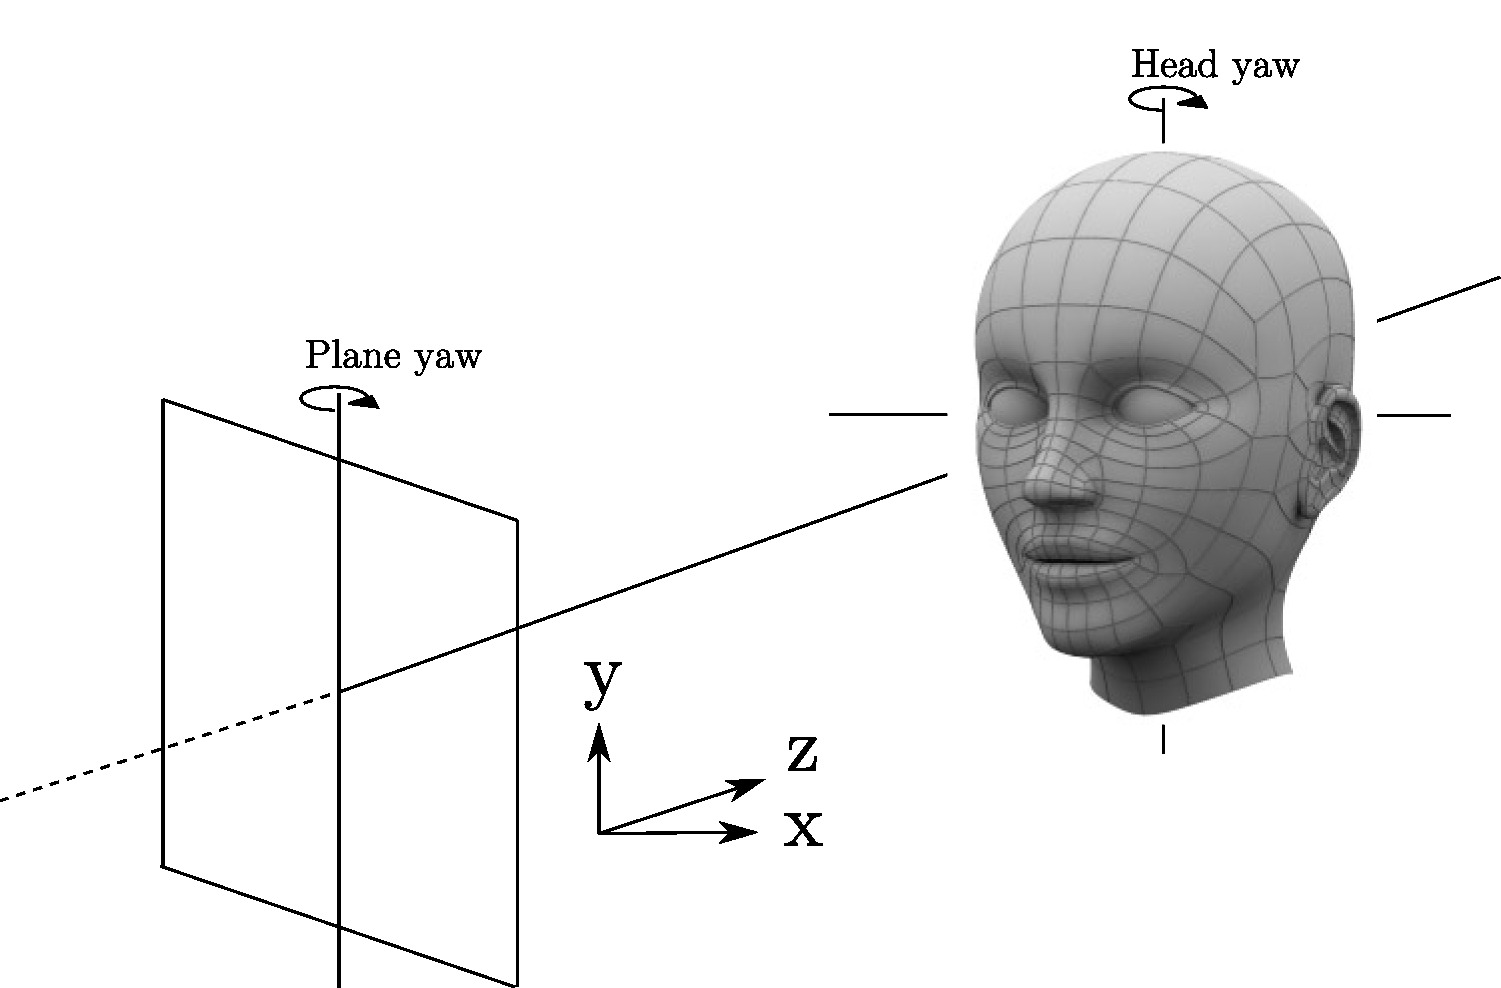
\includegraphics[bb=0 0 269 177]{images/planeyaw.jpg}
\end{figure}

\subsection{Fronto-parallel plane with constant distance from observer}
We want to show a plane of random dots with constant distance $l$ from the subject eyes and with its normal vector always parallel to the subject line-of-sight, like it would be on the tip of a rod stick with head.
The center of the stimulus is then obtained as
$$ \mathbf{x}_c(t) = \mathbf{p}_{c}(t) + l \left( \tilde{\mathbf{R}}(t) \cdot (0,0,-1)^T \right) $$
where $\mathbf{p}_c$ are the coordinates of the cyclopean eye, i.e. the average between the two eyes coordinates.
The stimulus rotation matrix is then simply the head transformation rotation matrix $\tilde{\mathbf{R}}$, so the final transformation to apply to an axis-aligned centered object is the following:
\begin{equation}
\mathbf{M}_s =   \begin{pmatrix}
  \tilde{\mathbf{R}} & \mathbf{x}_c \\
  \mathbf{0} & 1 \\ 
  \end{pmatrix}
\end{equation}



\bibliographystyle{alpha}
\bibliography{biblio}
\end{document}
